\section{Motivation}
\label{sec:motivation}

We present our ideas in the context of a DSL embedded in OCaml that
manages an abstract database state that can be manipulated via a
well-defined \C{SQL} interface. Arbitrary database computations can be
built around this interface, which can then be run as transactions
using the \C{atomically\_do} combinator provided by the DSL.

\begin{figure}[!t]
\centering
\begin{ocaml}
let new_order (d_id, c_id, item_reqs) = atomically_do @@ fun () ->
  let dist = SQL.select1 District (fun d -> d.d_id = d_id) in
  let o_id = dist.d_next_o_id in
  begin
    SQL.update(* UPDATE *) District 
              (* SET *)(fun d -> {d with d_next_o_id = d.d_next_o_id + 1})
              (* WHERE *)(fun d -> d.d_id = d_id );
    SQL.insert(* INSERT INTO *) Order (* VALUES *){o_id=o_id;  
              o_d_id=d_id; o_c_id=c_id; o_ol_cnt=S.size item_reqs; };
    foreach item_reqs @@ fun item_req ->
      let stk = SQL.select1(* SELECT * FROM *) Stock 
                (* WHERE *)(fun s -> s.s_i_id = item_req.ol_i_id &&
                                     s.s_d_id = d_id)(* LIMIT 1 *) in
      let s_qty' = if stk.s_qty >= item_req.ol_qty + 10 
                  then stk.s_qty - item_req.ol_qty 
                  else stk.s_qty - item_req.ol_qty + 91 in
      SQL.update Stock (fun s -> {s with s_qty = s_qty'}) 
                       (fun s -> s.s_i_id = item_req.ol_i_id);
      SQL.insert Order_line {ol_o_id=o_id; ol_d_id=d_id; 
                             ol_i_id=item_req.ol_i_id; ol_qty=item_req.ol_qty}
  end
 
\end{ocaml}
\caption{TPC-C \C{new\_order} transaction}
\label{fig:new_order_code}
\vspace*{-10pt}
\end{figure}

Fig.~\ref{fig:new_order_code} shows a simplified version of the TPC-C
\C{new\_order} transaction written in this language. TPC-C is a
widely-used and well-studied Online Transaction Processing (OLTP)
benchmark that models an order-processing system for a wholesale parts
supply business. The business logic is captured in 5 database
transactions that operate on 9 tables; \C{new\_order} is one such
transaction that uses \C{District}, \C{Order}, \C{New\_order},
\C{Stock}, and \C{Order\_line} tables. The transaction acts on the
behalf of a customer, whose id is \C{c\_id}, to place a new order for
a given set of items (\C{item\_reqs}), to be served by a warehouse
under the district identified by \C{d\_id}.  Fig.~\ref{fig:schema}
illustrates the relationship among these different tables.

The transaction manages order placement by invoking appropriate SQL
functionality, captured by various calls to functions defined by the
\C{SQL} module. All \C{SQL} operators supported by the module take a
table name (a nullary constructor) as their first argument. The
higher-order \C{SQL.select1} function accepts a boolean function that
describes the selection criteria, and returns any record that meets
the criteria (it models the SQL query \C{SELECT \ldots\xspace LIMIT
  1}). \C{SQL.update} also accepts a boolean function (its 3$^{rd}$
argument) to select the records to be updated. Its 2$^{nd}$ argument
is a function that maps each selected record to a new (updated)
record. \C{SQL.insert} inserts a given record into the specified table
in the database.

The \C{new\_order} transaction inserts a new \C{Order} record, whose
id is the sequence number of the next order under the given district
(\C{d\_id}). The sequence number is stored in the corresponding
\C{District} record, and updated each time a new order is added to the
system. Since each order may request multiple items (\C{item\_reqs}),
an \C{Order\_line} record is created for each requested item to relate
the order with the item. Each item has a corresponding record in the
\C{Stock} table, which keeps track of the quantity of the item left in
stock (\C{s\_qty}). The quantity is updated by the transaction to
reflect the processing of new orders (if the stock quantity falls below
10, it is automatically replenished by 91).

\begin{figure}[!t]
  \centering
	\begin{subfigure}{0.4\textwidth}
	  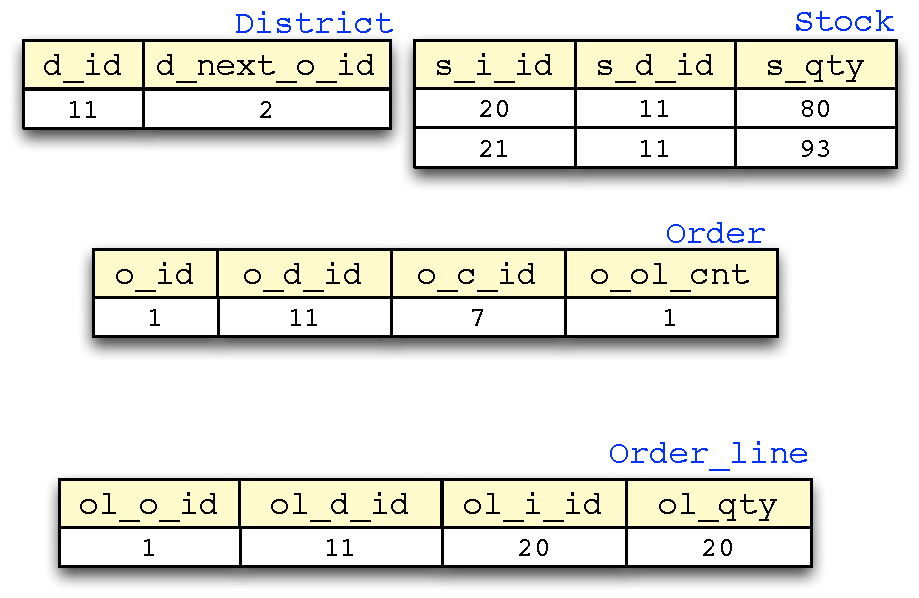
\includegraphics[width=0.9\textwidth]{Figures/schema1}
    \caption{A valid TPC-C database. The only existing order belongs
      to the district with \C{d\_id}=11. Its id (\C{o\_id}) is one
      less than the district's \C{d\_next\_o\_id}, and its order
      count (\C{o\_ol\_cnt}) is equal to the number of order line
      records whose \C{ol\_o\_id} is equal to the order's id.  }
		\label{fig:tpcc_db1}
	\end{subfigure}
  \hspace*{.2in}
	\begin{subfigure}{0.52\textwidth}
		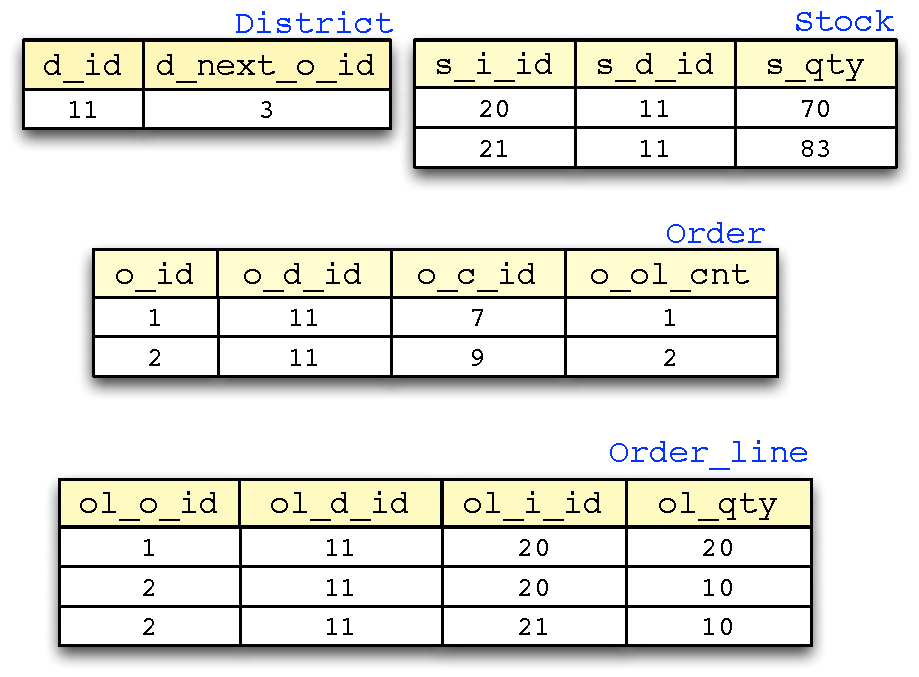
\includegraphics[width=0.9\textwidth]{Figures/schema2}
    \caption{The database in Fig.~\ref{fig:tpcc_db1} after correctly
      executing a \C{new\_order} transaction. A new order record is
      added whose \C{o\_id} is equal to the \C{d\_next\_o\_id} from
      Fig.~\ref{fig:tpcc_db1}. The district's \C{d\_next\_o\_id} is
      incremented. The order's \C{o\_ol\_cnt} is 2, reflecting the
      actual number of order line records whose \C{ol\_o\_id} is equal
      to the order's id (2).}
		\label{fig:tpcc_db2}
   	\end{subfigure}
\caption{Database schema of TPC-C's order management system.
  The naming
  convention indicates primary keys and foreign keys. For e.g.,
  \C{ol\_id} is the primary key column of the order line table,
  whereas \C{ol\_o\_id} is a foreign key that refers to the \C{o\_id}
  column of the order table.}
\label{fig:schema}
\end{figure}

TPC-C defines multiple invariants, called \emph{consistency
  conditions}, over the state of the application in the database. One
such consistency condition is the requirement that for a given order
\C{o}, the \emph{order-line-count} field (\C{o.o\_ol\_cnt}) should
reflect the number of order lines under the order; this is the number
of \C{Order\_line} records whose \C{ol\_o\_id} field is the same as
\C{o.o\_id}.  In a sequential execution, it is easy to see how this
condition is preserved.  A new \C{Order} record is added with its
\C{o\_id} distinct from existing order ids, and its \C{o\_ol\_cnt} is
set to be equal to the size of the \C{item\_reqs} set. The \C{foreach}
loop runs once for each \C{item\_req}, adding a new \C{Order\_line}
record for each requested item, with its \C{ol\_o\_id} field set to
\C{o\_id}. Thus, at the end of the loop, the number of \C{Order\_line}
records in the database (i.e., the number of records whose
\C{ol\_o\_id} field is equal to \C{o\_id}) is guaranteed to be equal
to the size of the \C{item\_reqs} set, which in turn is equal to the
\C{Order} record's \C{o\_ol\_cnt} field; these constraints ensure that
the transaction's consistency condition is preserved.

Because the aforementioned reasoning is reasonably simple to perform
manually, verifying the soundness of TPC-C's consistency conditions
would appear to be feasible.  Serializability aids the tractability of
verification by preventing any interference among concurrently
executing transactions while the \C{new\_order} transaction executes,
essentially yielding serial behaviors.  
\begin{wrapfigure}{l}{.4\textwidth}
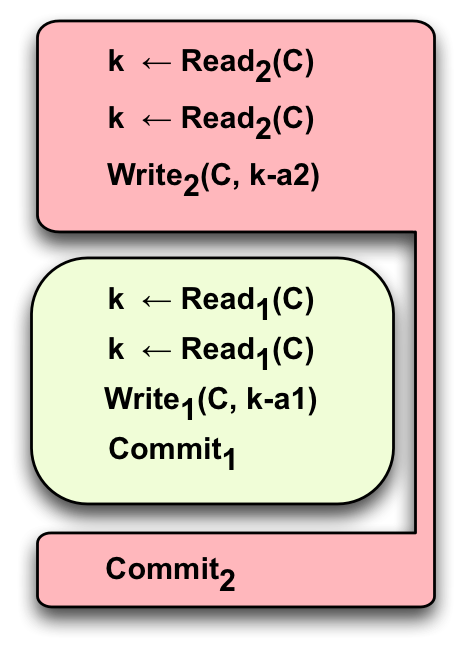
\includegraphics[scale=0.45]{Figures/motiv-eg-1-b}
\caption{\small An RC execution involving two instances ($T_1$ and
  $T_2$) of the \C{new\_order} transaction depicted in
  Fig.~\ref{fig:new_order_code}. 
  Both instances read the \C{d\_id} \C{District} record concurrently,
  because neither transaction is committed when the reads are
  executed.  The subsequent operations are effectively sequentialized,
  since $T_2$ commits before $T_1$. Nonetheless, both transactions read the same value for
  \C{d\_next\_o\_id} resulting in them  adding \C{Order} records
  with the same ids, which in turn triggers a violation of TPC-C's
  consistency condition.}
\label{fig:new_order_exec}
\vspace*{-10pt}
\end{wrapfigure}
Under weak isolation\footnote{Weak isolation does not violate
  atomicity as long as the witnessed effects are those of committed 
transactions}, however, interferences of various kinds are permitted,
leading to executions superficially similar to executions permitted by
concurrent (racy) programs~\cite{GHE15,HPQ+15}.  To illustrate,
consider the behavior of the \C{new\_order} transaction when executed
under a \emph{Read Committed} (RC) isolation level, the default
isolation level in 8 of the 18 databases studied
in~\cite{bailishotos}.  An executing RC transaction is isolated from
\emph{dirty writes}, i.e., writes of uncommitted transactions, but is
allowed to witness the writes of concurrent transactions as soon as
they are committed.  Thus, with two concurrent instances of the
\C{new\_order} transaction (call them $T_1$ and $T_2$), both
concurrently placing new orders for different customers under the same
district (\C{d\_id}), RC isolation allows the execution shown in
Fig.~\ref{fig:new_order_exec}.


% \begin{figure}[!h]
% \centering
% \subcaptionbox {
%   {\sc rc} Execution 1
%   \label{fig:motiv-eg-1-b}
% } [
%   0.55\columnwidth
% ] {
%   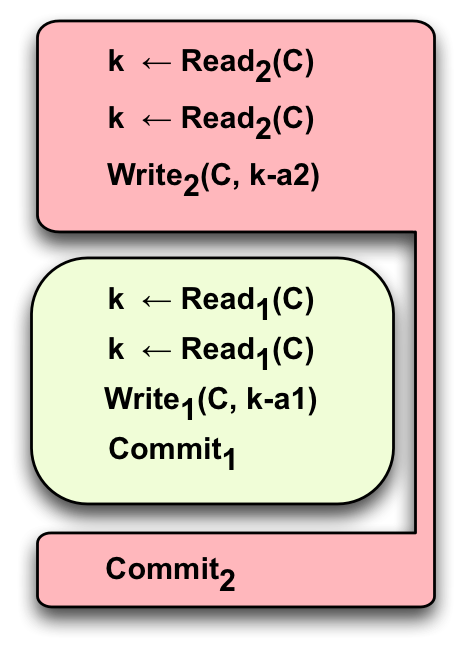
\includegraphics[scale=0.45]{Figures/motiv-eg-1-b}
% }
% %\hspace*{0.5in}
% \subcaptionbox {
%   {\sc rc} Execution 2
%   \label{fig:motiv-eg-1-a}
% }{
%   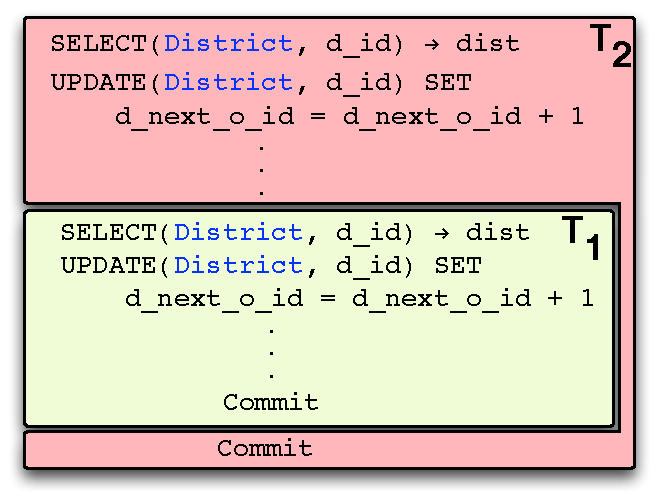
\includegraphics[scale=0.45]{Figures/motiv-eg-1-a}
% }
%   \caption{\small RC executions involving two instances ($T_1$ and
%   $T_2$) of the \C{new\_order} transaction depicted in
%   Fig.~\ref{fig:new_order_code}. 
%   Each instance reads the \C{d\_id} \C{District} record twice, the second
%   time to (atomically) update the \C{d\_next\_o\_id} field.}
% \label{fig:new_order_execs}
% \end{figure}

The figure depicts an execution as a series of SQL operations. In the
execution, the \C{new\_order} instance $T_1$ (green) reads the
\C{d\_next\_o\_id} field of the district record for \C{d\_id}, but
before it increments the field, another \C{new\_order} instance
$T_2$ (red) begins its execution and commits. Note that $T_2$ reads the
same \C{d\_next\_o\_id} value as $T_1$, and inserts new \C{Order} and
\C{Order\_line} records with their \C{o\_id} and \C{ol\_o\_id} fields
(resp.) equal to \C{d\_next\_o\_id}. $T_2$ also increments the
\C{d\_next\_o\_id} field, which $T_1$ has already acccessed. This is
allowed because reads typically do not obtain a mutually exclusive
lock on most databases. After $T_2$'s commit, $T_1$ resumes execution
and adds new \C{Order} and \C{Order\_line} fields with the same order
id as $T_1$. Thus, at the end of the execution, \C{Order\_line}
records inserted by $T_1$ and $T_2$ all bear the same order id. There
are also two \C{Order} records with the same district id (\C{d\_id})
and order id, none of whose \C{o\_ol\_cnt} reflects the actual number
of \C{Order\_line} records inserted with that order id.  This clearly
violates TPC-C's consistency condition.

This example does not exhibit any of the anomalies that
\emph{characterize} RC isolation~\cite{berenson}\footnote{Berenson
\emph{et al.} characterize isolation levels in terms of the anomalies
they \emph{admit}. For example, RC is characterized by \emph{lost
writes} because it admits the anomaly.}. For instance, there are no
\emph{lost writes} since both concurrent transactions' writes are
present in the final state of the database.  Program analyses that aim
to determine appropriate isolation by checking for possible
manifestations of RC-induced anomalies would fail to identify grounds
for promoting the isolation level of \C{new\_order} to something
stronger.  Yet, if we take the semantics of the application into
account, it is quite clear that RC is not an appropriate isolation
level for \C{new\_order}.

While reasoning in terms of anomalies is cumbersome and inadequate,
reasoning about weak isolation in terms of
traces~\cite{adyaphd,gotsmanconcur15} on memory read and write actions
can complicate high-level reasoning.  A possible alternative would be
to utilize concurrent program verification methods where the
implementation details of weak isolation are interleaved within the
program, yielding a (more-or-less) conventional concurrent program.
But, considering the size and complexity of real-world transaction
systems, this strategy is unlikely to scale.

In this paper, we adopt a different approach that \emph{lifts}
isolation semantics (\emph{not} their implementations) to the
application layer, providing a principled framework to simultaneously
reason about application invariants and isolation properties.  To
illustrate this idea informally, consider how we might verify that
\C{new\_order} is sound when executed under \emph{Snapshot Isolation}
(SI), a stronger isolation level than RC. Snapshot isolation allows
transactions to be executed against a private snapshot of the
database, thus admitting concurrency, but it also requires that there
not be any write-write conflicts (i.e., such a conflict occurs if
concurrently executing transactions modify the same record) among
concurrent transactions when they commit. Write-write conflicts can be
eliminated in various ways, e.g., through conflict detection followed
by a rollback, or through exclusive locks, or a combination of both.
For instance, one possible implementation of SI, close to the one used
by PostgreSQL~\cite{postgresiso}, executes a transaction against its
private snapshot of the database, but obtains exclusive locks on the
actual records in the database before performing writes. A write is
performed only if the record that is to be written has not already
been updated by a concurrent transaction. Conflicts are resolved by
abort and roll back.

%% This implementation is demonstrated for a simple
%% database with three records, $a$, $b$, and $c$ in
%% Fig.~\ref{fig:RR-postgres}.

%% \begin{figure}[t]
%% 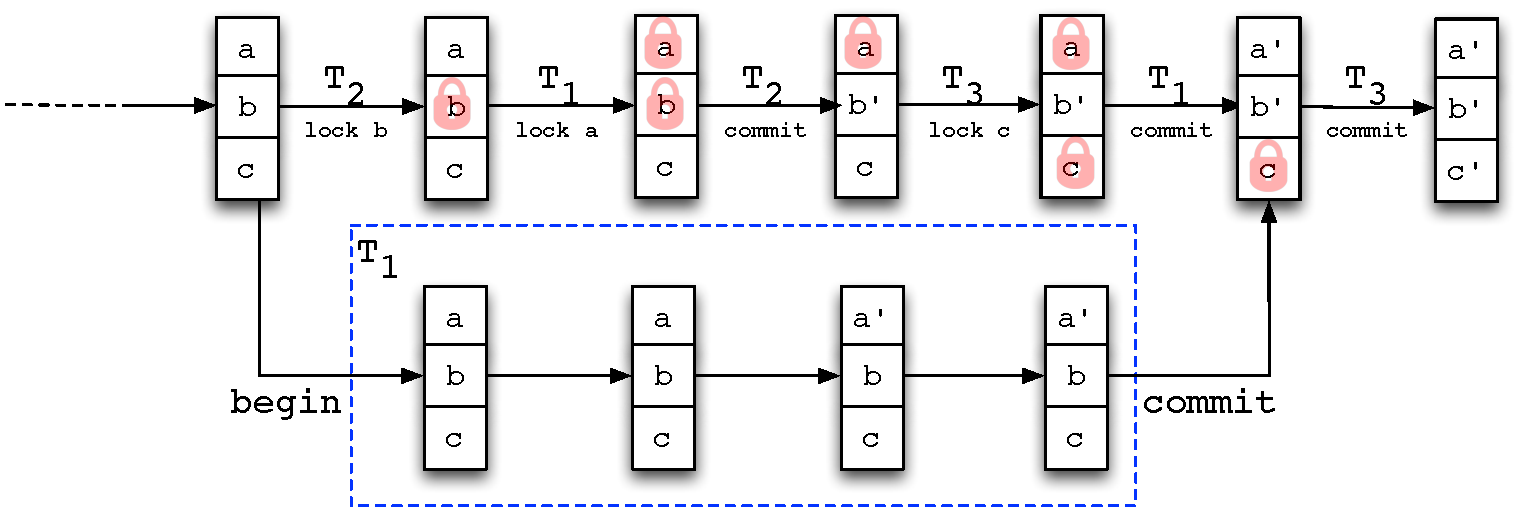
\includegraphics[scale=0.5]{Figures/RR-postgres}
%% \caption{Database state transitions corresponding to an execution of
%%   an SI transaction $T_1$ on a PostgreSQL-like store. $T_2$ and $T_3$
%%   are concurrent transactions. }
%% \label{fig:rr-postgres}
%% \end{figure}
%% \begin{figure}[t]
%% 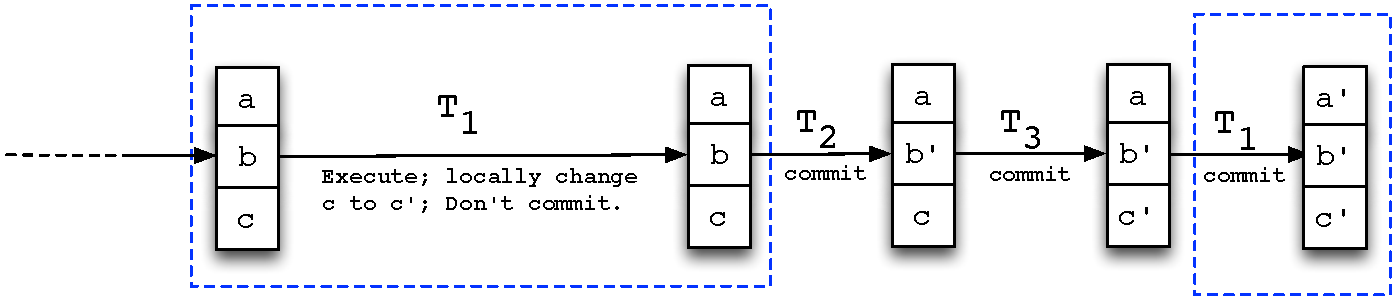
\includegraphics[scale=0.5]{Figures/RR-abstract}
%%   \caption{An abstract execution that includes the concrete execution
%%   shown in Fig.~\ref{fig:rr-postgres}. It has no locks or snapshots,
%%   admits fewer interleavings, yet results in the same post-state.  }
%% \label{fig:rr-abstract}
%% \end{figure}

As this discussion hints, implementations of SI on real databases
such as PostgreSQL are highly complicated, often running into
thousands of lines of code.  Nonetheless, the semantics of SI, in
terms of how it effects transitions on the database state, can be
captured in a fairly simple model. First, effects induced by one
transaction (call it $T$) are not visible to another concurrently executing one
during $T$'s execution. Thus, from $T$'s perspective,
the global state does not change during its execution.  More formally,
for every operation performed by $T$, the global state $T$ witnesses
before ($\stg$) and after ($\stg')$ executing the operation is the
same ($\stg'=\stg$).  After $T$ finishes execution, it commits its
changes to the actual database, which may have already incorporated
the effects of concurrent transactions. In executions where $T$
successfully commits, concurrent transactions are guaranteed to not be
in write-write conflict with $T$. Thus, if $\stg$ is the global state
that $T$ witnessed when it finished execution (the snapshot state),
and $\stg'$ is the state to which $T$ commits, then the difference
between $\stg$ and $\stg'$ should not result in a write-write conflict
with $T$. To concretize this notion, let the database state be a map
from database locations to values, and let $\stl$ denote a
transaction-local log that maps the locations being written to their
updated values.  The absence of write-write conflicts between $T$ and
the diff between $\stg$ and $\stg'$ can be expressed as: $\forall
x\in\mathit{dom}(\delta)$, $\stg'(x) = \stg(x)$.  In other words, the
semantics of SI can be captured as an axiomatization over transitions
of the database state ($\Delta \longrightarrow \Delta'$) during a
transaction's ($T$) lifetime:
\begin{itemize}
  \item While $T$ executes, $\Delta' = \Delta$.
  \item After $T$ finishes execution, but before it commits its local
    state $\delta$, $\forall(x\in\mathit{dom}(\delta)).~\Delta'(x) = \Delta(x)$.
\end{itemize}

% nor $T$'s effects are
% witnessed by concurrent transactions, during $T$'s execution. Thus,
% $T$'s execution can be thought of as a series of transitions of a
% state local to $T$ (call it $\stl$), that has no bearing outside $T$. Conversely, any
% transitions performed by the concurrent transactions on the global
% state (call it $\stg$) has no
% bearing on $T$ since $T$ reads off a static snapshot established at
% the beginning of the transaction. Consequently, any
% state transitions performed by the concurrent transactions can be
% \emph{moved past} $T$'s local state transitions. $T$'s commit,
% however, is a global state transition that is enabled only if
% there are no WW conflicts between $T$ and concurrent transactions.
% Thus, concurrent transactions' state transitions cannot be moved past
% $T$'s commit, and $T$ can be thought of witnessing the effects of
% concurrent transactions just before its commit. 
% therefore treat Since a
% transaction's reads are always served from a snapshot, no state
% changes are witnessed while the execution is in progress. Thus,
% insofar as an RR transaction is concerned, the database state does not
% change during the execution.  Uncommitted writes are recorded in a
% transaction-local state.  When the transaction commits, the local
% state is atomically written to the global state to yield a global
% state that reflects the transaction's updates.  However, unlike a
% strongly isolated serializable transaction, the commit operation is
% performed against the current state of the database, not the
% snapshot. Thus, after the transaction finishes execution, but before
% it commits, the transaction is able to witness the effects of all
% concurrent transactions that committed before it.  The PostgreSQL RR
% implementation effectively constrains this transition.

% We can axiomatize this operational description by observing that (a)
% due to the version check, the current transaction cannot update a data
% item that was already updated by a concurrent transaction, and (b) due
% to the use of exclusive write locks, a data item updated by the
% current transaction cannot be overwritten by a concurrent transaction.
% If $\Delta$ is the state of the database when an RR transaction
% finishes, and $\Delta_c$ is the state visible to the transaction at
% the point of commit, we know the transition from $\Delta$ to
% $\Delta_c$ (written $\Delta \longrightarrow \Delta_c$) cannot exhibit
% effects from any concurrent transactions that write to the same data
% items as the current RR transaction.  Similarly, if $\delta$ denotes
% a local log that relates transaction variables being written with their updated values,
% then $\forall x\in\mathit{dom}(\delta)$, $\Delta_c(x) =
% \Delta(x)$. To summarize, the operational semantics of PostgreSQL's RR
% implementation can be captured as an axiomatization over transitions of
% the database state ($\Delta \longrightarrow \Delta'$) during the
% lifetime an RR transaction ($T$):
% \begin{itemize}
%   \item While $T$ executes, $\Delta' = \Delta$.
%   \item After $T$ finishes execution, but before it commits its local
%     state $\delta$, $\forall(x\in\delta).~\Delta'(x) = \Delta(x)$.
% \end{itemize}

\noindent This simple characterization of SI isolation allows us to
verify the consistency conditions associated with the \C{new\_order}
transaction.  First, since the database does not change ($\Delta' =
\Delta$) during execution of the transaction's body, we can reason
about \C{new\_order} as though it executed in complete isolation until
its commit point, leading to a verification process similar to what
would have been applied when reasoning sequentially.  When
\C{new\_order} finishes execution, however, but before it commits, the
SI axiomatization shown above requires us to consider global state
transitions $\stg \longrightarrow \stg'$ that do not include changes
to the records ($\stl$) written by \C{new\_order}, i.e.,
$\forall(x\in\mathit{dom}(\delta)).~\Delta'(x) = \Delta(x)$.  The
axiomatization precludes any execution in which there are concurrent
updates to shared table fields (e.g., \C{d\_next\_o\_id} on the same
\C{District} table), but does not prohibit interferences that write to
different tables, or write to different records in the same table.  We
need to reason about the safety of such interferences with respect to
\C{new\_order}'s consistency invariants to verify \C{new\_order}.

%% Since concurrent
%% \C{new\_order} transactions that write to the same \C{District} record
%% modify the record by incrementing its \C{d\_next\_o\_id} field, their
%% transitions do not satisfy the necessary condition imposed by the SI
%% axiomatization, allowing us to rightfully ignore their interference.
%% This leaves the interference due to concurrent \C{new\_order}
%% transactions that write to a different district record.  Fortunately,
%% such interference does not prompt \C{new\_order} to violate the
%% invariant, which can be established by adopting a reasoning similar to
%% the one used on concurrent program logics, such as the Rely-Guarantee
%% logic, customized for the database programs.

% and becomes ready to commit, a
% transition transfers the transaction's local writes ($\delta$) to the
% unchanged database state ($\Delta$).  However, we are required to
% consider the interference from concurrent transitions at this point,
% which might change the database state from $\Delta$ to $\Delta_c$. If
% this interference includes the effects of a concurrent \C{new\_order}
% transaction (with the same \C{d\_id}), then verification fails as
% described previously.  Fortunately, sequential reasoning shows that
% this is impossible - RR prevents a concurrent \C{new\_order}
% transaction that modifies the same \C{District} record as the current
% transaction (concretely, since the record is already present in the
% current transaction's local log, any transition from $\Delta$ to
% $\Delta_c$ cannot change this record).  Applying such axiomatic
% reasoning on \C{new\_order} allows us to prove that the TPC-C
% invariant holds when the transaction is executed under PostgreSQL's RR
% isolation.  Our proof framework generalizes this style of reasoning to
% various isolation levels on databases.

%% The second observation that informs our approach is one that pertains
%% to automation. Program verification, even when machine-aided, often
%% entails significant annotation burden in the form of intermediary
%% assertions and loop invariants required to prove a program correct.
%% This is certainly true for concurrent program logics, such as
%% Rely-Gurantee, which extend Hoare logic with additional artifacts and
%% where (stable) intermediary assertions and loop invariants remain a
%% major source of annotation burden.

We approach the verification problem by first observing that a
relational database is a significantly simpler abstraction than shared
memory. Its primary data structure is a table, with no primitive
support for pointers, linked data structures, or aliasing.  Although a
database essentially abstracts a mutable state, this state is managed
through a well-defined fixed number of interfaces (SQL statements),
each tagged with a logical formula describing what records are
accessed and updated.

This observation leads us away from thinking of a collection of
database transactions as a simple variant of a concurrent imperative
program.  Instead, we see value in viewing them as essentially
functional computations that manage database state abstractly,
mirroring the structure of our DSL.  By doing so, we can formulate the
semantics of database operations as state transformers that explicitly
relate an operation's pre- and post-states, defining the semantics of
the corresponding transformer algorithmically, just like classical
predicate transformer semantics (e.g., weakest pre-condition or
strongest post-condition).  In our case, a transformer interprets a
SQL statement in the set domain, modeling the database as a set of
records, and a SQL statement as a function over this set.  Among other
things, one benefit of this approach is that low-level loops can now
be substituted with higher-order combinators that automatically lift
the state transformer of its higher-order argument, i.e., the loop
body, to the state transformer of the combined expression, i.e., the
loop.  We illustrate this intuition on a simple example.


%% Thus the semantics of a \C{foreach} loop, for instance, can be
%% captured as a state transformer, where the state is a set, and the
%% transformation defines a bind operation.

% \begin{figure}[!t]
% \centering
% %
% \begin{subfigure}[b]{0.46\textwidth}
% \begin{ocaml}
% Set s' = $\emptyset$;
% foreach x in s {
%   s'.add(f(x)); 
% }
% \end{ocaml}
% \caption{}
% \end{subfigure}
% %
% \begin{subfigure}[b]{0.5\textwidth}
% \begin{ocaml}
% let s' = ref [];
% foreach s (fun x -> s' := x::(!s'));
% \end{ocaml}
% \caption{Lorem ipsum, lorem ipsum,Lorem ipsum, lorem ipsum,Lorem ipsum}
% \end{subfigure}
% \caption{Caption place holder}
% %
% \caption{New versions are created from existing versions either
% through \C{push} or \C{merge}.}
% \label{fig:syntactic-ancestors}
% \end{figure}
% let s' = ref (Set.empty) in
% foreach xs @@ fun x -> 
%   begin
%     s' := Set.union !s' @@ 
%             Set.map_selected s (fun y -> y<x)
%                                (fun y -> y+x);
%     s' := Set.add !s' x;
%   end
\begin{figure}[!h]
\begin{ocaml}
foreach item_reqs @@ fun item_req ->
  SQL.update Stock (fun s -> {s with s_qty = k1}) 
                   (fun s -> s.s_i_id = item_req.ol_i_id);
  SQL.insert Order_line {ol_o_id=k2; ol_d_id=k3; 
                         ol_i_id=item_req.ol_i_id; ol_qty=item_req.ol_qty}
\end{ocaml}
\caption{Foreach loop from Fig.~\ref{fig:new_order_code}}
\label{fig:foreach_code}
\end{figure}

Fig.~\ref{fig:foreach_code} shows a (simplified) snippet of code taken
from Fig.~\ref{fig:new_order_code}. Some irrelevant expressions have
been replaced with constants (\C{k1}, \C{k2}, and \C{k3}).  The body of
the loop executes a SQL update followed by an insert.  Recall that a
transaction reads from the global database ($\Delta$), and writes to a
transaction-local database ($\delta$) before committing these
updates. An update statement filters the records that match the search
criteria from $\Delta$ and computes the updated records that are to be
added to the local database. Thus, the state transformer for the
update statement (call it $\T_U$) is the following function on
sets\footnote{Bind ($\bind$) has higher precedence than union
($\cup$). Angle braces ($\langle \ldots \rangle$) are used to denote
records.}:
\begin{smathpar}
\begin{array}{l}
  \lambda(\stl,\stg).~ \stl \cup \stg \bind(\lambda \C{s}. 
      \itel{{\sf table}(\C{s}) = \C{Stock} \conj 
        \C{s}.\C{s\_i\_id} = \C{item\_req.ol\_i\_id}\\\hspace*{1.15in}}
           {\{ \langle \C{s\_i\_id}=\C{s.s\_i\_id};\, 
                       \C{s\_d\_id}=\C{s.s\_d\_id};\,
                       \C{s\_qty} = \C{k1}\rangle \}\\\hspace*{1.15in}}
           {\emptyset})
\end{array}
\end{smathpar}
% \begin{smathpar}
% \begin{array}{c}
%   \lambda\Delta.\lambda\delta.\, \delta \;\cup\; 
%       \Delta \,\bind\, (\lambda s.\, 
%           \C{if}\;{\C{stock}(s) \conj 
%                    \C{s.s\_i\_id} = \C{item\_req.ol\_i\_id}}\\
%            \hspace*{0.9in}
%            \C{then}\;{\{\{s \;\C{with}\; \C{s\_qty} = \C{k1}\}\}}\;
%            \C{else}\;{\emptyset})
% \end{array}
% \end{smathpar}
% \begin{verbatim}
%   Rmem(σ'(s')) = Rmem(σ(s')) U 
%                  Rmem[\x. Rmem[\y. if y<x then {y+x} else {}](σ(s)) U {x}](xs)
% \end{verbatim}
% Observe that
% $\T_U(\Delta,\delta)$ is of the form $\delta \,\cup\,
% F_U(\Delta)$.
Here, the set bind operator extracts record elements ($\C{s}$) from
the database, checks the precondition of the update action, and if
satisfied, constructs a new set containing a single record that is
identical to $\C{s}$ except that it binds field $\C{s\_qty}$ to value
$\C{k_1}$.  This new set is added (via set union) to the existing
local database state $\delta$.\footnote{For now, assume that the
  record being added is not already present in $\stl$.}

The transformer ($\T_I(\delta,\Delta)$) for the subsequent \C{insert}
statement can be similarly constructed:
\begin{smathpar}
\begin{array}{l}
  \lambda(\stl,\stg).~ \stl \cup
       \{\langle\C{ol\_o\_id}=\C{k2};\,
                 \C{ol\_d\_id}=\C{k3};\, \C{ol\_i\_id}=\C{item\_req.ol\_i\_id};\, 
                 \C{ol\_qty}=\C{item\_req.ol\_qty}\rangle\}
 
\end{array}
\end{smathpar}
Observe that both transformers are of the form $\T(\delta,\Delta) =
\stl \cup \F(\stg)$, where $\F$ is a function that returns the
set of records added  to the transaction-local database ($\stl$). Let
$\F_U$ and $\F_I$ be the corresponding functions for $\T_U$ and $\T_I$
shown above. The state transformation induced by the loop body in
Fig.~\ref{fig:new_order_code} can be expressed as the following
composition of $\F_U$ and $\F_I$:
\begin{smathpar}
\begin{array}{l}
  \lambda(\stl,\stg).~ \stl \cup \F_U(\stg) \cup \F_I(\stg)
\end{array}
\end{smathpar}
The transformer for the loop itself can now be computed to be:
\begin{smathpar}
\begin{array}{l}
  \lambda(\stl,\stg).~ \stl \cup \C{item\_reqs}\bind
      (\lambda\C{item\_req}.~ \F_U(\stg) \cup \F_I(\stg))
\end{array}
\end{smathpar}
Observe that the structure of the transformer mirrors the structure of
the program itself. In particular, SQL statements become set
operations, and the \C{foreach} combinator becomes set monad's bind
($\bind$) combinator.  As we demonstrate, the advantage of inferring
such transformers is that we can now make use of a
semantics-preserving translation from the domain of sets equipped with
$\bind$ to a decidable fragment of first-order logic, allowing us to
leverage SMT solvers for automated proofs without having to infer
potentially complex thread-local invariants or intermediate
assertions.  Sec.~\ref{sec:inference} describes this translation. In
the exposition thus far, we assumed $\Delta$ remains invariant, which
is clearly not the case when we admit concurrency.  Necessary
concurrency extensions of the state transformer semantics to deal with
interference is also covered in Sec.~\ref{sec:inference}.  Before
presenting the transformer semantics, we first focus our attention in
the following two sections on the theoretical foundations for weak
isolation, upon which this semantics is based.
